\section{The Bayesian Network Reasoner}
\label{BNReasoner}

A Bayesian Network (BN), as stated above, is a probabilistic graphical model where each node corresponds to a random variable and each edge represents the conditional probability for the corresponding variables. A BN corresponds to a directed acyclic graph (DAG) and to a set of conditional probability tables (CPTs), which, for every value \textbf{x} of variable \textbf{X} and every instantiation \textbf{u} \textbf{U}, define the Pr(\textbf{x}$\mid$\textbf{u}). 

\intextsep
\begin{figure}[H]
    \centering
    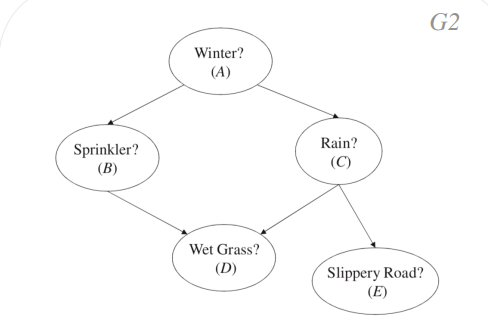
\includegraphics[width=0.45\textwidth]{Assets/BN example1.png}
    \hfill
    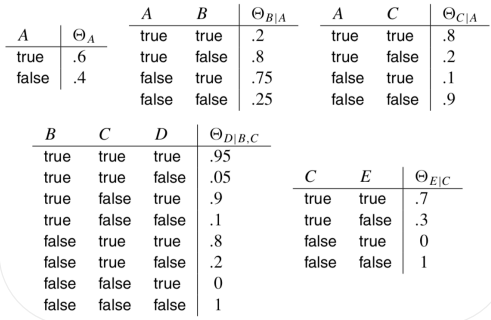
\includegraphics[width=0.45\textwidth]{Assets/BN example2.png}
    \caption{BN example}
    \label{fig:my_label}
\end{figure}

The Bayesian Network Reasoner has been implemented using the following algorithms:

\subsubsection{d-Separation:} %The structure of a Bayesian Network is interpreted as declaring a number of independence statements and probabilistic independence satisfies the graphoid axioms. 
One can derive new independencies to the independencies declared in the structure using d-separation. According to d-separation variable \textbf{X} are d-separated from variable \textbf{Y} by variables \textbf{Z} if every path from node \textbf{X} to node \textbf{Y} is blocked by \textbf{Z}. \textbf{X} and Y are d-separated by \textbf{Z} in DAG \textit{G} if and only if the graphoid axioms can be used to show that \textbf{X} and \textbf{Y} are independent given \textbf{Z}.  
\\
This graphical test was implemented by first pruning (i.e. deleting) all leaf nodes in the graph that are not part of the union of \textbf{X}, \textbf{Y} and \textbf{Z}. Then all edges outgoing from the variables in \textbf{Z} are removed. Finally, a recursive function iterates through all variables in X and their neighbours and calls itself for every neighbour while keeping track of the variables that have been visited in a set, these are skipped. It returns $True$ when it comes across a variable in \textbf{Y}, since this means that \textbf{X} and \textbf{Y} are connected, otherwise it returns $False$ when it has iterated through all variables connected to \textbf{X}. The output of the d-seperation function is then the opposite of the aforementioned recursive function, since two variables are d-seperated by Z when they are not connected after the pruning steps mentioned above.

\subsubsection{Ordering:} In solving a query, we apply variable elimination to remove the variables which are not relevant to answer the query. Given an interaction graph \textbf{G} and variable \textbf{X} to eliminate, we obtain \textbf{G'} adding an edge between every pair of neighbours of \textbf{X} that are not already connected by an edge, we delete \textbf{X} from \textbf{G}, multiply all factors containing \textbf{X} and finally sum-out \textbf{X} from the resulting factor. The order in which variables are eliminated is important and two heuristics can be used: 

\paragraph{min-degree:} always choose the node with the smallest degree. The way that this has been implemented is by creating the interaction graph of the network and iterating through each node while counting the number of edges and adding the node with the smallest number (which is the degree) to the list. 

\paragraph{min-fill:} always choose the node whose elimination adds the smallest number of edges. The implementation of this function first creates an interaction graph of the network and then computes for each node how many edges would be added if this node were to be deleted (this is done by counting how many of the node's parents are not connected to each other). The node with the lowest value is then added to the list.

\subsubsection{Network Pruning:} Network pruning is done through Node Pruning and Edge Pruning. With node pruning, given a BN \textbf{N} and a query (\textbf{Q,e}), we can remove any leaf node from \textbf{N} as long as it does not belong to variables \textbf{Q U e}. With edge pruning, for each edge from node \textbf{U} to \textbf{X}, we can remove the edge from \textbf{N} and replace the CPT of $\Theta$X $\mid$ U by a smaller CPT obtained from  $\Theta$X $\mid$ U assuming the value \textit{u} of \textbf{U} given in evidence \textit{e}.

\subsubsection{Marginal Distributions:} Given two variables \textbf{X} and \textbf{Y}, their marginal distribution is their joint probability distribution. We define \textbf{prior marginal} as our prior belief about the value of variable \textbf{X}, while we refer to \textbf{posterior marginal} as our knowledge about variable \textbf{X} having observed variable \textbf{Y}. 

\subsubsection{MAP and MPE:} MAP (Most a Posteriori Hypothesis) and MPE (Most Probable Explanation) refers to two types of queries representing the most likely instantiations (i.e. truth value assignments) of the variables in the network. 
%MAP queries refers to the most likely instantiation of variables given the evidence. MPE queries consider the most likely instantiation of the variables excluding the evidence. 
While both MAP and MPE compute this query based on evidence (given variable assignments), MAP focuses on a subset of variable instantiations, while MPE computes the most likely assignment of each variable.
The specific method for eliminating a variable depends on the query, for example, to solve the condition probability the variables have to be summed out. To solve an MPE problem we eliminate the variables by maxing them out while a MAP query requires both summing-out and maxing-out.   









